\documentclass{article}
\usepackage[utf8]{inputenc}
\usepackage{graphicx}
\usepackage[english]{babel}
\usepackage{csquotes}
\usepackage{hyperref}
\hypersetup{
    colorlinks=true,
    linkcolor=blue,
    filecolor=magenta,      
    urlcolor=cyan,
}

\title{{\Huge CS699- Software Lab Project Report on Hindi Text to Speech }}
\author{\Large Saurabh Warade- 193050051\\
\Large  Sanjay Kumar - 193050068}
\date{November 2019}

\begin{document}

\maketitle

\thispagestyle{empty}
\newpage

\clearpage
\pagenumbering{arabic}
\tableofcontents
\newpage

\section {Introduction}

\large Speech processing technology has been a mainstream 
area of research for more than 50 years. The ultimate 
goal of speech research is to build systems that mimic (or 
potentially surpass) human capabilities in understanding, 
generating and coding speech for a range of human-tohuman and human-to-machine interactions.\par
Speech is one of the most vital forms of communication in 
our everyday life. Since speech is a primary medium for 
communication among human beings, it is natural for the 
people to expect to be able to carry out spoken dialogue 
with computers. This involves the integration of speech 
technologies and language technologies. Speech synthesis 
is an automatic generation of artificial speech signal by 
the computer. In the last few years, this technology has 
been widely available for several languages for different 
platform from personal computer to stand alone system. 
Today, the most common interfaces for human machine 
interaction are still keyboards, keypads, and mice. 
However, an increasing necessity to interface with 
machines in mobile environments is leading to speech 
becoming a required means to interface with machines 
and automated information services.\par
TTS is a complex problem that has made significant progress in the realm of 
concatenative systems in the last few years.With the 
development of new techniques such as speech synthesis 
and speech recognition, we are now moving into an era of 
more effective TTS with improved prosody in the 
synthesize speech. Developing a text to speech system for 
a language that can support inputs in other languages can 
be helpful to the users who know the language but are not 
familiar with its relative keyboard layout. Users who do 
not know that language at all can type in that language 
using their local language keyboard layout. Many times,
Indian users prefer to type Hindi sentences in English 
Script. This fact is more prevalent over mobile SMS 
application, chatting and the social networking websites. 
Users do this because they are used to the English 
QWERTY keyboard and due to non-familiarity and nonavailability of the Hindi keyboard.

\bigskip

Based on the scenario as above, the need for an effective 
TTS system for Hindi Language is highly felt which 
implemented to provide an option to the user to input the
text either in Devnagri script or in Romanized English 
text. For such a system input string comes in form of a 
Romanized sentence or word (all possibilities considered) 
apart from the regular Hindi sentence or word, which is 
further processed to output a synthesized speech.
\bigskip


\newpage

\begin{figure}[htp]
    \centering
    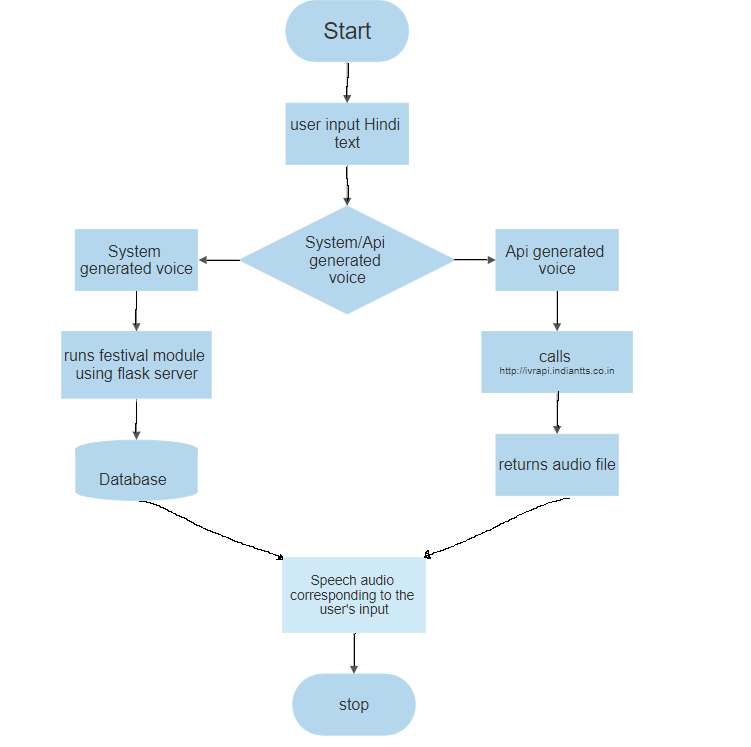
\includegraphics[width=14cm]{flow}
    \caption{Project flow}
    \label{fig:flow.PNG}
\end{figure}

\newpage
\section{Goals}

\begin{itemize}
    \item \textbf \Large {Generate system generated Voice of Hindi Text (Male Voice)}
    
       \large We take the input text from the user in Devanagari fonts and using the festival module we use it's (voice hindi NSK diphone) functionality to generate the voice corresponding to the text entered. 
    \item \textbf \Large {Generate API generated Voice of Hindi Text (Female Voice)}
        
        \large We use API of \cite{indianTTS}www.indiantts.co.in to generate audio corresponding to the input either in Hindi, Hinglish or English language.  
    \item \textbf \Large {To improve the model using “Transfer Learning”}
        
        \large We use the Transfer Learning because it allows us to build accurate models in a time-saving way. With transfer learning, instead of starting the learning process from scratch, you start from patterns that have been learned when solving a different problem. This way you leverage previous learnings and avoid starting from scratch.
   
\end{itemize}

\newpage
\section{Methodology}

\large The TTS for Hindi uses the widely used \cite{festival} Festival 
TTS engine. The text analysis module part converts all 
non standard words to standard ones. The phonemic 
analysis module is a grapheme-to-phoneme converter,
converting the written text into a sequence of 
phonemic symbols. The prosodic analysis module then
takes the phoneme sequence, and assigns to each 
phoneme the required pitch and duration. Both the 
129
phonemic and prosodic analyses are typically language 
dependent. Then the final the speech synthesis is 
performed by using two different concatenative 
synthesis techniques available in the Festival engine –
unit selection and multisyn unit selection. We 
implemented all the modules using Festival tools.

\newpage
\section{DESIGN AND IMPLEMENTATION OF TTS}


\quad \large A text-to-speech system is composed of two parts: a frontend and a back-end. The front-end has two major tasks. \par
\bigskip
First, it converts raw text containing symbols like 
numbers and abbreviations into the equivalent of writtenout words. This process is often called text normalization, 
pre-processing, or tokenization. The front-end then 
assigns phonetic transcriptions to each word, and divides 
and marks the text into prosodic units, like phrases, 
clauses, and sentences. The back-end—often referred to 
as the synthesizer – then converts the symbolic linguistic 
representation into sound, by a concatenative 
approach.The user writes the text either in Devnagri or 
Romanized script of Hindi language.The written text is 
processed only in Romanized script but also adaptable for 
Devnagri script. Such system for Hindi language is only 
possible when Devnagri is converted to Romanized script. 
Once the Romanized script is obtained, the task of text 
analysis and speech generation of TTS system is done.
In order to develop a TTS system, the bottom down 
approach deals with the designing of database.\par
\bigskip
Preparing a database is the main theme of any TTS system. The 
database is designed purely on Hindi language but 
represented in Romanized script for the ease of platform 
compatibility. The database is formed by preparing 
various phonemes of Hindi language.A word document is 
interfaced by the user to write Devnagri script.


\newpage

\section{Work Done:}

\subsection{Web application:}
\large We have created web application using \cite{w3schools}HTML, JAVASCRIPT, CSS, BOOTSTRAP.
\begin{itemize}
    \item \large HTML is used for making Web-page
    \item \large JAVASCRIPT is used for API connection of www.indiantts.co.in
    \item \large CSS is used for making GUI attractive
    \item \large BOOTSTRAP is used for Designing
\end{itemize}

\subsection{Server creation using Python Flask:}

\large \cite{stackoverflow}Flask is a micro web framework written in Python. It is classified as a micro framework because it does not require particular tools or libraries. It has no database abstraction layer, form validation, or any other components where pre-existing third-party libraries provide common functions.\par

We used flask for running Festival module in Ubuntu and passing commands.

\bigskip

\subsection{Training the Festival module using Transfer Learning:}
\large Transfer Learning is used to train the Festival module using data available online from IIT-Madras. 

\bigskip
\newpage
\textbf{FILES:}
\begin{enumerate}
    \item \Large We have main file entry point server.py (can be run as)
    
    \begin{displayquote}
        \textit{python3 server.py}
    \end{displayquote}
    
    \item \Large Two UI files in folders Static & Templates 
        \begin{enumerate}
            \item Static: 
                contains file style.css
            \item Templates: 
                contains file index.html
        \end{enumerate}
    
\end{enumerate}

\large Link to access data: \url{https://github.com/srwarade/CS699}


\newpage


\subsection{Challenges}
\begin{itemize}
    \item \large We didn't have the text conversion facility which directly converts input text to Hindi text. For this we need to convert the text to Hindi using GOOGLE Translate and then paste it to the input box.\par
    this problem is incurred only for System generated voice and using API we need not to do this conversion.

    \item \large We are unable to get enough training data for Hindi to train Festival module, which resulted in Robotic voice as output.
    
    \item \large The system generated voice uses System resources heavily which causes lag in the system resulting in inconsistency.
    
    \item \large The Flask Server in python is storing a file in the drive of the user's input to pass it as input to the Festival module.
\end{itemize}

% Fraction of time spent in different parts of the project.  
% What was the most challenging part?
% Fraction of work done by different team members.


\begin{thebibliography}{9}
\bibitem{w3schools}
w3schools
\\\texttt{https://www.w3schools.com}
 
\bibitem{stackoverflow}
Stackoverflow
\\\texttt{https://www.stackoverflow.com}. 

\bibitem{festival}
Festival
\\\texttt{https://www.festvox.org/festival}

\bibitem{indianTTS}
IndianTTS
\\\texttt{https://www.indiantts.com}

\end{thebibliography}
\end{document}
